\documentclass{article}

\usepackage{amsmath}
\usepackage{color}
\usepackage[hidelinks]{hyperref}
\usepackage{listings}
\usepackage{tikz}
\usepackage{tikz-qtree}
\usepackage{verbatim}

% Colors copied from https://stackoverflow.com/questions/3175105/
\definecolor{dkgreen}{rgb}{0,0.6,0}
\definecolor{gray}{rgb}{0.5,0.5,0.5}
\definecolor{mauve}{rgb}{0.58,0,0.82}

\lstset{
	aboveskip=5mm,
	belowskip=5mm,
	basicstyle={\large\ttfamily},
	columns=flexible,
	language=Lisp,
	numbers=left,
	showstringspaces=false,
	% Style copied from https://stackoverflow.com/questions/3175105/
	numberstyle=\normalsize\color{gray},
	keywordstyle=\color{blue},
	commentstyle=\color{dkgreen},
	stringstyle=\color{mauve},
}

\bibliographystyle{acm}

\title{The Ergonomics of Faceted Execution (full draft)}
\author{Ian Fisher}
\date{17 April 2019}

\begin{document}
\maketitle

\begin{abstract}
	This thesis draft reviews faceted execution, a programming-language mechanism for enforcing privacy policies. I discuss several issues with the use of faceted execution in real-world software development (efficiency, type safety, compatibility with non-faceted code), and review methods of mitigating these issues (abstract interpretation, static typing, Racket's \texttt{\#lang} mechanism). I present a proof-of-concept of a module-rewriting technique that could be used to improve the existing \textsc{Racets} system \cite{racets} for faceted execution in Racket.
\end{abstract}

\tableofcontents



\section{Introduction}
\subsection{Faceted execution\label{sec:facets}}
Software applications often require that access to some data is governed by a privacy policy. On a social media website, for instance, a user's contact information may only be visible to the user's friends, while their name and profile picture may be public. Beyond social media, in sectors like banking and healthcare the proper enforcement of privacy policies has serious legal and ethical consequences. However, implementing privacy policies in code can be tedious and error-prone, as the privacy logic tends to become coupled to the application logic. Faceted execution is a programming-language mechanism that aims to ease the implementation of privacy policies by decoupling an application's privacy policy from its logic.

Faceted execution allows privacy policies to be expressed separately from the implementation of the program, meaning that changes to the privacy policy can be made reliably with minimal modification of the application logic. Faceted execution is thus an implementation of policy-agnostic programming \cite{faceted}.

The keystone of faceted execution is the use of special data structures called facets. A facet is a tuple of the form $\langle l\ ?\ v_H : v_L \rangle$ where $l$ is a label, $v_H$ is the high-confidentiality value, and $v_L$ is the low-confidentiality value. $v_H$ can only be accessed by observers that match the facet's label; other observers see only $v_L$, which is typically a default value like $0$ or \texttt{null}. A special function must be called to explicitly observe the value of the facet; otherwise, the facet behaves just like a regular value.

Full support of faceted execution requires changes to core language mechanisms like function application. Concretely, if the (facet-unaware) function \texttt{square-root} were applied to the facet $\langle l \ ?\ 42 : 0 \rangle$, it must return the facet $\langle l \ ?\ \texttt{square-root}(42) : \texttt{square-root}(0) \rangle$, ensuring that the faceted value remains protected by the privacy policy, even if \texttt{square-root} is totally oblivious to the policy. Without changes to the mechanics of function application, a privacy-agnostic version of \texttt{square-root} would either choke on faceted input (since it expects an integer), inadvertently reveal sensitive data, or both.

Researchers have adopted different strategies to implement faceted execution. One strategy is to design a new programming language with faceted-execution primitives built-in. This is the strategy adopted by the Jeeves programming language \cite{jeeves}. Another strategy is to use syntactic macros to graft faceted execution on to an existing language, provided that the language's macro system is rich enough to support it. The \textsc{Racets} programming language adopts the latter strategy, by augmenting the Racket language with syntactic macros \cite{racets}.

The following subsections will present an overview of the mechanics of faceted execution specific to the \textsc{Racets} programming language, but the concepts are general enough to apply to other implementations of faceted execution.


\subsubsection{A simple example of faceted execution}
Policies, which govern access to sensitive data, are declared with the \texttt{let-label} form in \textsc{Racets}:

\begin{lstlisting}
(define alice-policy
  (let-label l (lambda (x) (equal? x "Alice")) l))

(define bob-policy
  (let-label l (lambda (x) (equal? x "Bob")) l))
\end{lstlisting}

The two declarations in the source code above create two policies and bind them to the names \texttt{alice-policy} and \texttt{bob-policy}. Note the somewhat idiomatic usage of the \texttt{let-label} form: the general syntax is \texttt{(let-label name value body)}, which binds \texttt{name} to \texttt{value} and evaluates \texttt{body} with this new binding. In the two declarations above, the body is simply the label name itself, so that the \texttt{let-label} form as a whole creates and then returns the label.

The policies enforce that only entities identifying themselves as ``Alice'' or ``Bob'', respectively, may view the high-confidentiality value of any facet protected by the policies.

A faceted data value is created with the \texttt{fac} form:

\begin{lstlisting}
(define my-facet (fac alice-policy 42 0))
\end{lstlisting}

\texttt{my-facet} is defined with Alice's policy, the high-confidentiality value $42$, and the low-confidentiality value $0$.

The \texttt{obs} form is used to view the value of a facet:

\begin{lstlisting}
(obs alice-policy "Alice" my-facet)
\end{lstlisting}

The expression above will evaluate to $42$, as the argument \texttt{"Alice"} satisfies the facet's policy. By contrast, the expression below will evaluate to $0$ since \texttt{"Bob"} does not satisfy the facet's policy.

\begin{lstlisting}
(obs alice-policy "Bob" my-facet)
\end{lstlisting}

The policy passed to a facet must match the policy that the facet was created with. In the case that the facets do not match, \texttt{obs} functions as a no-op. Each of the two calls to \texttt{obs} below, for instance, will return \texttt{my-facet} unchanged, since \texttt{my-facet} uses Alice's policy and not Bob's.

\begin{lstlisting}
(obs bob-policy "Alice" my-facet)
(obs bob-policy "Bob" my-facet)
\end{lstlisting}

The forms \texttt{let-label}, \texttt{fac}, and \texttt{obs} comprise the primitive operations of faceted execution in \textsc{Racets}.


\subsubsection{An example of nested facets}
Faceted values may be nested for more finely-grained control over the views of the data that are available. While a single facet only encloses two different views of the data, a nested facet may enclose an arbitrary number of views. Alice could define a nested facet that specifies her location in three degrees of granularity:

\begin{lstlisting}
(define location-facet
  (fac alice-policy
    "370 Lancaster Ave, Haverford PA"
    (fac bob-policy
      "Haverford, PA"
      "Pennsylvania")))
\end{lstlisting}

Alice is able to view the full street address of her location. Bob (or anyone else satisfying Bob's policy) may see her town, and anyone else may only see her state of residence. The structure of the nested facet may be visualized as a tree, where the left branches are the high-confidentiality values, the right branches are the low-confidentiality values, the leaves are the non-faceted values, and the internal nodes are the policies. Figure \ref{figure:nested} represents the facet defined above.

\begin{figure}[h]
\begin{center}
	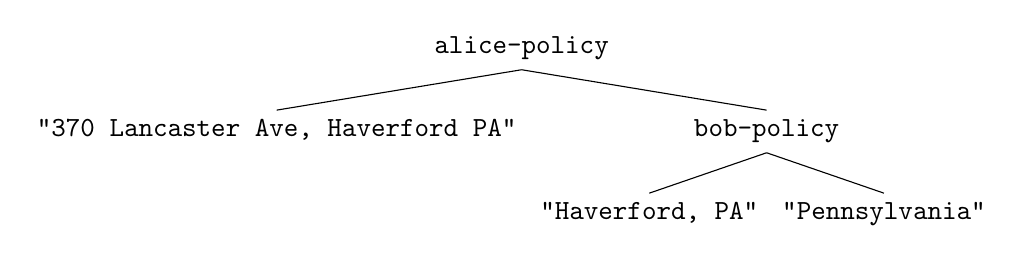
\begin{tikzpicture}
	\Tree
	[.\texttt{alice-policy}
		\texttt{"370 Lancaster Ave, Haverford PA"}
		[.\texttt{bob-policy}
			\texttt{"Haverford, PA"}
			\texttt{"Pennsylvania"}
		]
	]
	\end{tikzpicture}
	\caption{A nested facet}
	\label{figure:nested}
\end{center}
\end{figure}

Alice observes her nested facet in the usual way:

\begin{lstlisting}
(obs alice-policy "Alice" location-facet)
\end{lstlisting}

Bob must make two calls to \texttt{obs} to fully resolve the facet's value:

\begin{lstlisting}
(obs alice-policy "Bob" (obs bob-policy "Bob" location-facet))
\end{lstlisting}

As before, Bob must ensure that the policy he passes to each \texttt{obs} call matches the policy of the facet. In this case, the outer facet uses Alice's policy and the inner facet uses Bob's policy, so the calls to \texttt{obs} must be organized likewise.


\subsubsection{An example of faceted structs}
Compound data structures such as Racket structs may be faceted. However, their behavior is somewhat counterintuitive. Take the following example:

\begin{lstlisting}
(struct employee (name position salary))
(define bob
  (employee "Bob" "manager" (fac bob-policy 70000 0)))
\end{lstlisting}

The call to the \texttt{employee} constructor is handled by \textsc{Racets} the same way that any function call is: by branching execution on both values on the facet. Therefore, the return value is \texttt{(fac bob-policy (employee "Bob" "manager" 70000) (employee "Bob" "manager" 0))}, i.e. a facet that wraps two different instantiations of the \texttt{employee} struct, rather than a structure containing a faceted value for the \texttt{salary} field, as one might expect. Bob's faceted salary can be accessed like so:

\begin{lstlisting}
(employee-salary (obs bob-policy "Bob" bob))
; or, equivalently:
(obs bob-policy "Bob" (employee-salary bob))
\end{lstlisting}

Somewhat surprisingly, \texttt{obs} is required to observe the name field (and any other field) of the \texttt{employee} object, even though it was not explicitly faceted in the constructor.

\begin{lstlisting}
(employee-name (obs bob-policy "Bob" bob))
\end{lstlisting}

\textsc{Racets} programs must take care to address these subtleties when working with faceted structs.


\subsubsection{An example of faceted lists}
Using faceted values with lists involves additional complications. Consider the following example:

\begin{lstlisting}
(define grades (list))
(set! grades (cons (fac alice-policy 84 0) grades))
\end{lstlisting}

Similarly to the example with structs, the programmer likely intended for \texttt{grades} to be of the form \texttt{(list (fac alice-policy 84 0))}, i.e. a regular list containing a single facet. However, the real value of \texttt{grades} after the \texttt{set!} operation is

\begin{lstlisting}
(fac alice-policy (list 84) (list 0))
\end{lstlisting}

Imagine another grade was added to the list, like so:

\begin{lstlisting}
(set! grades (cons (fac bob-policy 73 0) grades))
\end{lstlisting}

Then the value of the list would be

\begin{lstlisting}
(fac bob-policy
  (fac alice-policy (list 73 84) (list 73 0))
  (fac alice-policy (list 0 84) (list 0 0)))
\end{lstlisting}

\noindent encompassing four different possibilities: satisfying both Alice and Bob's policies, satisfying one or the other, or satisfying neither. The tree in figure \ref{figure:nested-list} illustrates this structure diagrammatically.

\begin{figure}[h]
\begin{center}
	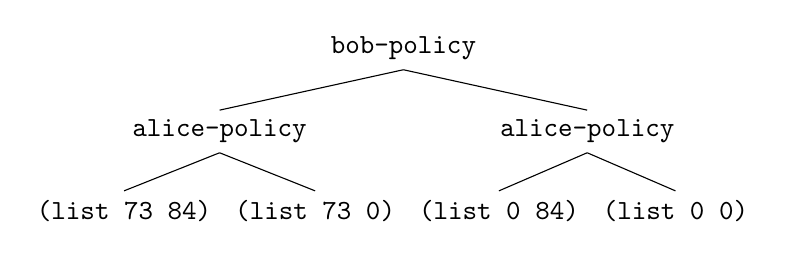
\begin{tikzpicture}
		\Tree
		[.\texttt{bob-policy}
			[.\texttt{alice-policy}
				\texttt{(list 73 84)}
				\texttt{(list 73 0)}
			]
			[.\texttt{alice-policy}
				\texttt{(list 0 84)}
				\texttt{(list 0 0)}
			]
		]
	\end{tikzpicture}
	\caption{A nested facet containing lists}
	\label{figure:nested-list}
\end{center}
\end{figure}

Programmers may find it useful to convert a list of facets into a regular Racket list. \texttt{reveal-grades-rec} accomplishes this:

\begin{lstlisting}
(define (reveal-grades-rec grade-list policy-list arg)
  (if (empty? policy-list)
    grade-list
    (obs
      (car policy-list)
      arg
      (reveal-grades-rec
        grade-list
        (cdr policy-list)
        arg))))])
\end{lstlisting}

\texttt{reveal-grades-rec} takes in a list of grades, a list of policies which should correspond index-by-index to the list of grades (remember that \texttt{obs} requires the policy to match the facet's policy), and an argument to pass to the policy predicates. It traverses the policy tree tail-recursively, observing a single policy at each step.

This section and the previous one have illustrated fundamental issues with the interaction of faceted execution and data structures, stemming from the generic treatment of faceted function application. For the sake of programming ergonomics, future implementations of faceted execution may wish to not treat functional application quite so generically, to allow structure-creating forms like \texttt{list} and struct constructors to be special cases that behave more intuitively with faceted arguments.


\subsection{Syntactic macros}
The implementation of faceted execution in \textsc{Racets} relies on a language feature called syntactic macros. Syntactic macros are a mechanism by which the source syntax of a program is transformed prior to execution. They are a more powerful cousin of the lexical macros familiar to C and C++ programmers. Racket, like most dialects of Lisp, includes a particularly powerful syntactic macro system. Since macros figure heavily in the implementation of \textsc{Racets}, a brief introduction to the Racket macro system is given here. Readers are referred to the ``Fear of Macros'' tutorial \cite{fear-of-macros} for a much more comprehensive treatment.

A macro is defined like a function that takes a syntax object as input and outputs another syntax object, except the definition uses \texttt{define-syntax} instead of \texttt{define}. The simplest possible macro returns its input syntax unchanged:

\begin{lstlisting}
(define-syntax (identity stx)
  stx)
\end{lstlisting}

A macro is invoked just like a regular function:

\begin{lstlisting}
; Expands to just x
(identity x)
\end{lstlisting}

New syntax objects can be constructed with the \texttt{syntax} function or its abbreviation, \texttt{\#'}:

\begin{lstlisting}
(define-syntax (ignore-input stx)
  ; Equivalent to (syntax (displayln "ignoring input"))
  #'(displayln "ignoring input")
\end{lstlisting}

Syntax objects can be converted to and from lists. This functionality allows us to implement a macro that reverses its arguments:

\begin{lstlisting}
(define-syntax (reverse-syntax stx)
  (datum->syntax stx (reverse (cdr (syntax->datum stx)))))
\end{lstlisting}

A programmer could use the \texttt{reverse-syntax} macro as follows:

\begin{lstlisting}
; Expands to (+ 20 22), which evaluates to 42
(reverse-syntax 20 22 +)
\end{lstlisting}

\texttt{reverse-syntax} is the first example of a macro that could not be written as a regular Racket function, since it actually effects a transformation of the source syntax. Another example, familiar to users of the C preprocessor, accesses the location information that syntax objects carry to dynamically print the location of the macro invocation in the source code.\footnote{A similar effect can be achieved using the C preprocessor with the \texttt{\_\_LINE\_\_} and \texttt{\_\_FILE\_\_} macros.}

\begin{lstlisting}
(define-syntax (print-source-location stx)
  (datum->syntax
    stx
    `(displayln
       (format
         "line ~a of ~a"
         ,(syntax-line stx)
         ,(syntax-source stx)))))
\end{lstlisting}

More complicated macros can be written with the pattern-matching facilities of \texttt{syntax-case}. The following macro uses \texttt{syntax-case} to behave differently if it invoked with one argument or two:

\begin{lstlisting}
(define-syntax (one-or-two stx)
  (syntax-case stx ()
    [(_ a b)
     #'(displayln "Got two")]
    [(_ a)
     #'(displayln "Got one")]))
\end{lstlisting}

In the snippet above, each identifier in the \texttt{syntax-case} clause matches a single top-level expression (which may be an atomic value or a compound structure like a list). The underscore matches the name of the macro itself,\footnote{The use of an underscore is purely conventional, to indicate that the macro does not carry about the value it captures. Racket itself treats it the same as any other identifier in a syntax pattern.} and the symbols \texttt{a} and \texttt{b} match arguments to the macro.

One final point about syntactic macros in Racket is that they are hygienic, meaning that identifiers introduced in the macro are protected from conflicting with identifiers in the original source code. Consider the following macro:

\begin{lstlisting}
(define-syntax (hygienic stx)
  (syntax-case stx ()
    [(_ a)
     #'(let ([x 10]) (+ x a))]))
\end{lstlisting}

If \texttt{hygienic} was used in a context where another identifier \texttt{x} was defined, e.g.

\begin{lstlisting}
(define x 32)
(hygienic x)
\end{lstlisting}

then one might expect that it would expand to

\begin{lstlisting}
; Wrong!
(define x 32)
(let ([x 10] (+ x x)))
\end{lstlisting}

which would (counterintuitively) evaluate to 20. In actual fact, the macro system rewrites the identifier \texttt{x} in the macro to a name which it can guarantee will not collide with any existing identifier in the program, as demonstrated below.

\begin{lstlisting}
; Correct -- x in the macro is rewritten as x:3
(define x 32)
(let ([x:3]) (+ x x:3))
\end{lstlisting}

At runtime the expanded macro thus correctly evaluates to 42.

By contrast, macros in C are not hygienic, so in \texttt{swap} below, the \texttt{tmp} variable defined in the macro will interfere with unrelated uses of \texttt{tmp} in the same scope as the macro invocation.

\begin{lstlisting}[language=C]
#define swap(x, y) int tmp = x; x = y; y = tmp;
\end{lstlisting}

Hygienic syntactic macros are a powerful feature of the Racket language that will be leveraged in section \ref{sec:lang} to implement faceted execution in a seamless manner that would not be possible in a language that did not expose a rich set of mechanisms for language extension.



\section{Extending Racket with faceted execution\label{sec:lang}}
The current implementation of \textsc{Racets} is consists of a collection of syntactic macros. I will review the current implementation, and then present a more flexible and powerful approach using Racket's \texttt{\#lang} mechanism, as well as a concrete proof-of-concept illustrating a crucial technique for using \texttt{\#lang}.


\subsection{Racets with macros}
The \textsc{Racets} macros redefine core Racket constructs like \texttt{lambda}, \texttt{if}, and \texttt{\#\%app} (function application) to make them sensitive to faceted values. For example, the \texttt{lambda} form is transformed by the \texttt{fac-lambda} macro, which wraps the resulting function in a special data structure.

\begin{lstlisting}
(define-syntax (fac-lambda stx)
  (syntax-parse stx
    [(_ xs expr)
      #'(fclo (lambda xs expr))]))
\end{lstlisting}

Other macros are provided for a subset of the core forms of Racket. See \cite{racets} for details of the implementation.


\subsubsection{Shortcomings}
Implementing \textsc{Racets} using macros suffers from two shortcomings: certain constructions involving \texttt{set!} are not (and cannot be) handled correctly, and the \textsc{Racets} macros may interfere with user-defined macros.

To correctly handle \texttt{set!} forms with faceted values, the \textsc{Racets} system needs to wrap (some) identifiers with the \texttt{facet-deref} form. To see why, consider the following code snippet:

\begin{lstlisting}
(if k
  (set! x 100)
  (set! x 0))
\end{lstlisting}

Suppose that \texttt{k} is a facet belonging to Alice whose high-confidentiality value is true and whose low-confidentiality value is false. Upon execution of the \texttt{if} statement, the value of \texttt{x} will be a box that contains the facet $\langle \textit{alice}\ ?\ 100 : 0 \rangle$. However, subsequent references to \texttt{x} will assume that it is of integer type, and without a \texttt{facet-deref} transformation to extract the underlying facet from the box, these references may cause the code fail.

Note that this is a different problem from invisibly transforming regular values into facets, as was done in many of the examples of section \ref{sec:facets}. Faceted values are automatically handled by the faceted execution mechanism, e.g. the re-defining of the \texttt{\#\%app} macro to work for facets. The problem here is that the use of the \texttt{set!} form (which expands to \texttt{facet-set!} in \textsc{Racets}) results in \texttt{x} becoming a box containing a facet and not just a bare facet.

It is simply not possible to target bare identifiers with a syntactic macro because identifiers are ``raw'' in the syntax: unlike function applications, lambda definitions, and other Racket forms, identifiers are not wrapped in an identifier-specific syntactic form at any point in the macro expansion process, and thus it is impossible for a macro to target them specifically and exclusively, at least not in the way that, e.g., \texttt{\#\%app} can target every function application.


\subsection{Racets as a language-as-a-library}
These shortcomings can be averted with \textsc{Racets}'s \texttt{\#lang} mechanism. Source files in Racket typically begin with a \texttt{\#lang racket} declaration. However, other languages may be defined (e.g., \texttt{\#lang typed/racket} \cite{typed-racket}) which reuse some of the syntax and semantics of Racket and modify other parts of it. The semantics, syntax, and even lexical structure can be altered using \texttt{\#lang}.

The language-as-a-library approach \cite{typed-racket} uses \texttt{\#lang} to implement new domain-specific languages which are compatible with plain Racket code and which are much easier to write than an entire new language, since they can reuse all the facilities exposed by the Racket compiler.

The key idea of languages-as-libraries is to override the \texttt{\#\%module-begin} form (which wraps all Racket modules), and use a Racket function called \texttt{local-expand} to simplify the module's contents into a minimal subset of Racket called Fully-Expanded Racket \cite{fe-racket}. The language designer then need only provide translations for the small set of core forms that constituted Fully-Expanded Racket.


\subsubsection{Small example of a language-as-a-library}
The following minimal but complete example of the languages-as-libraries idea prints out the fully-expanded abstract syntax tree of a program before running it normally:

\begin{lstlisting}
#lang racket

; Fully expands the module and prints out its abstract syntax
; tree, before running it normally.
(define-syntax (module-begin stx)
  (syntax-case stx ()
    [(_ forms ...)
    (with-syntax ([(_ core-forms ...)
                   (local-expand
                     #'(#%plain-module-begin forms ...)
                     'module-begin
                     '())])
      #'(#%plain-module-begin
          (displayln '(core-forms ...))
          core-forms ...))]))

; Export everything from the regular Racket language, except
; replaced #%module-begin with our own implementation.
(provide (except-out (all-from-out racket) #%module-begin)
  (rename-out [module-begin #%module-begin]))
\end{lstlisting}

If this program were saved in a file called \texttt{racket/print-ast.rkt}, then other files could be written in the language by beginning with \texttt{\#lang s-exp "racket/print-ast.rkt"} instead of \texttt{\#lang racket}.

The file \texttt{racket/print-ast.rkt} begins with the standard \texttt{\#lang racket} declaration, since the file itself is written in Racket. It then defines a macro called \texttt{module-begin} which rewrites its syntax object to be

\begin{lstlisting}
#'(#%plain-module-begin
    (displayln '(core-forms ...))
    core-forms ...))]))
\end{lstlisting}

where \texttt{core-forms} is defined by the \texttt{with-syntax} clause to be the result of invoking \texttt{local-expand} on the original syntax object. The macro then outputs a \texttt{\#\%plain-module-begin} form (rather than a \texttt{\#\%module-begin}, to avoid infinite recursion) that wraps the original source syntax, after a call to \texttt{displayln} that prints at run-time the actual syntax object that was generated at compile-time.


\subsubsection{Larger example of a language-as-a-library}
As a proof-of-concept of implementing Racets with the language-as-a-library approach, this section presents a library called \texttt{wrap-ident.rkt} that rewrites identifiers in the source code in roughly the manner that the real \textsc{Racets} implementation requires.

\begin{lstlisting}
#lang s-exp "wrap-ident.rkt"

(define x 10)
(define y 32)
(displayln (+ x y))
\end{lstlisting}

The effect of the \texttt{wrap-ident.rkt} module is to re-write the syntax tree as follows:

\begin{lstlisting}
(define x 10)
(define y 32)
(displayln ((var-wrapper +) (var-wrapper x)
                               (var-wrapper y)))
\end{lstlisting}

where \texttt{var-wrapper} is defined as

\begin{lstlisting}
(define (var-wrapper v)
  (if (and (box? v) (facet? (unbox v)))
    (unbox v)
    v))
\end{lstlisting}

The core of the \texttt{wrap-ident.rkt} module is the \texttt{transform-syntax} procedure, which recursively walks the program's syntax tree, detects bare identifiers, and wraps them with \texttt{var-wrapper}. Most forms in Fully-Expanded Racket can be transformed simply by recursively transforming each of sub-forms except for the first (which is typically a special identifier like \texttt{define} or \texttt{set!} that cannot be wrapped in a function call). Some forms need to be treated specially because their syntax forbids some of their subforms from being wrapped. An example is \texttt{set!}: if \texttt{(set! x 10)} were re-written as \texttt{(set! (var-wrapper x) 10)}, then Racket would give a syntax error as the first argument to \texttt{set!} must be a bare identifier. \texttt{transform-syntax} therefore contains several pattern matches for forms which must be treated specially, followed by a default case for any other list of forms, followed by a case for any individual form, which performs the actual work of identifying and re-writing identifiers.

\begin{lstlisting}
(define (transform-syntax stx)
  (syntax-case stx ()
    ; set!
    ([head id expr]
     (check-ident #'head #'set!)
     #`(head id #,(transform-syntax #'expr)))

    ; provide
    ([head a ...]
     (check-ident #'head #'#%provide)
     stx)

    ; #%plain-lambda
    ([head formals expr ...]
     (check-ident #'head #'#%plain-lambda)
     (datum->syntax stx
                    (cons #'head
                          (cons #'formals
                                (map transform-syntax
				     (syntax-e #'(expr ...)))))))

    ; quote
    ([head datum]
     (check-ident #'head #'quote)
     #'(head datum))

    ; Any other list of forms.
    ([a b ...]
     (datum->syntax stx (cons #'a (map transform-syntax
                                           (syntax-e #'(b ...))))))

    ; Any other individual form.
    (default
      (if (identifier? #'default)
        #`(var-wrapper #,#'default)
        #'default))))
\end{lstlisting}

The code listing above is not exhaustive: special cases are omitted for \texttt{let-values} and \texttt{letrec-values}, among others, as their syntax requires complex pattern matching.

Each pattern has a guard clause that uses the helper function \texttt{check-ident} to check that the head of the matched form is bound to the same variable as the form we intend to re-write. \texttt{check-ident} is defined below. It uses \texttt{free-identifier=?} to check its argument's binding. It is important to use this method and not simply compared the textual content of the identifiers because Racket does not guarantee these will be the same. For example, an identifier may have the surface form of \texttt{lambda} but actually be bound to \texttt{\#\%plain-lambda}. \texttt{free-identifier=?}, unlike an equality comparison, is sensitive to these distinctions.

\begin{lstlisting}
(define (check-ident ident expected)
  (and (identifier? ident) (free-identifier=? ident expected)))
\end{lstlisting}

The final piece is the whole-module rewrite rule:

\begin{lstlisting}
(define-syntax (module-begin stx)
  ; Intercept the entire module and transform it using
  ; `transform-syntax` on the fully-expanded syntax tree (which
  ; ensures that user macros are expanded first).
  (syntax-case stx ()
    [(_ forms ...)
     (let ([expanded
            (local-expand #'(#%plain-module-begin forms ...)
	                  'module-begin
			  '())])
       (transform-syntax expanded))]))

(provide (except-out (all-from-out racket) #%module-begin)
         (rename-out [module-begin #%module-begin]))
\end{lstlisting}

The \texttt{module-begin} macro invokes \texttt{local-expand} on the module contents, and then calls \texttt{transform-syntax} to transform the resulting fully-expanded syntax tree.



\section{Type theory}
Since the \textsc{Racets} language is dynamically typed, errors in the use of faceted values (such as supplying the wrong policy to \texttt{obs}) are not caught until runtime. A static type system for faceted values would be able to more reliably catch programmer errors.

The definition of a type system is ``a tractable syntactic method for proving the absence of certain program behaviors by classifying phrases according to the kinds of values they compute'' \cite{types}. The program behaviors that a type system are meant to prevent are generally what are called type errors: attempted operations on values for which the operation is not defined.

Naturally, some undesirable program behaviors cannot be detected by a static type system (e.g., looping infinitely is not detectable due to the uncomputability of the halting problem), and type systems will sometimes refuse to accept constructs which are in fact safe. Nonetheless, a well-designed type system is an effective tool for catching programmer errors.

A simple model of a static type system is the typed lambda-calculus. The following exposition is based on chapter 9 of \cite{types}.

The lambda calculus is a simple model of computation in which the only data type is the function and the only operation is function application. Syntactically the lambda calculus has three kinds of terms: variables ($x$, $y$, etc.), anonymous functions, also known as abstractions ($\lambda x . x$), and function applications ($t\ t$). The notation $\lambda x . x$ is equivalent to the more traditional notation of $f(x) = x$, with the advantage of not requiring the function to be named. Function application of the form $t_1\ t_2$ is equivalent notationally to $t_1(t_2)$, i.e. the application of the function $t_1$ to the argument $t_2$. The body of a lambda function may contain any of the three syntactic forms of the language, so for example $\lambda x . \lambda y . (\lambda z . z)(x)$ is a valid term in the lambda calculus whose outermost abstraction contains another abstraction, which in turn contains an application. For clarity, the application is wrapped in parentheses.

The typed lambda calculus has the same syntax as the untyped lambda calculus, except that a type annotation is necessary for lambda abstractions, which are now written as $\lambda x: T . x$, where $T$ is a type. The $: T$ syntax is an example of a \textit{type annotation}---an annotation supplied by the programmer that indicates the intended type of a variable or expression. Not all typed languages require type annotations, but they can be beneficial for clarity and simplicity of implementation.

A type system for the lambda calculus (and indeed for any programming language) must assign a type to each syntactic construction in the language. These assignments are formally known as type rules. Type rules are written in the form

\[
\frac{\text{hypotheses}}
{\text{conclusion}}
\]

\noindent where \textit{hypotheses} is a set of assumptions and \textit{conclusion} is a type judgment that follows from the hypotheses.

The rule for the types of variables is\footnote{The type rules are taken from Figure 9-1 on p. 103 of \cite{types}.}

\[
\frac{x : T \in \Gamma}
{\Gamma \vdash x : T}
\]

$\Gamma$ stands for an assignment function that maps from a finite number of variable names to their values. The notation $\Gamma \vdash t : T$ expresses the three-place typing relation that syntactic term $t$ has type $T$ given the assignment $\Gamma$. The type rule for variables simply states that if a variable is paired with a certain type $T$ in the assignment function, then $T$ is the variable's type.

The rule for lambda abstraction is a bit more complicated:

\[
\frac{\Gamma, x : T_1 \vdash t_2 : T_2}
{\Gamma \vdash \lambda x : T_1 . t_2 : T_1 \to T_2}
\]

In the hypothesis, the expression $\Gamma, x : T_1$ should be read as ``$\Gamma$ augmented with the assignment of type $T_1$ to $x$.'' It is assumed that the variable $x$ is not already in $\Gamma$; if it is, it can simply be renamed. The full hypothesis of the abstraction rule thus states that the body of the lambda function has type $T_2$ with the given assignment function. The conclusion of the abstraction rule states that the lambda function as a whole has the complex type $T_1 \to T_2$.

Finally, the last syntactic form of the language, application, has the type rule

\[
\frac{\Gamma \vdash t_1 : T_{11} \to T_{12}\ \ \ \ \ \ \Gamma \vdash t_2 : T_{11}}
{\Gamma \vdash t_1\ t_2 : T_{12}}
\]

Given that the function has type $T_{11} \to T_{12}$ in $\Gamma$, and the argument has type $T_{11}$, then the expression as a whole has type $T_{12}$.

The three type rules presented above can be applied to any expression in the typed lambda calculus to detect whether it is well-typed, and if it is, to determine its concrete type. Thus the type system is able to statically eliminate a class of errors from the simple lambda calculus.

Type systems for real programming languages are significantly more complex, but involve the same basic formalism of inference rules and type judgments. As such, this formalism could be deployed to augment \textsc{Racets} with a static type system that detects programming errors specific to faceted execution.



\section{Abstract interpretation}
Another practical problem of working with faceted execution is that it can have high runtime cost. As the example with \texttt{square-root} in section \ref{sec:facets} indicated, functions applied to facets must be evaluated twice, once with the high-confidentiality value and once with the low-confidentiality value. The double evaluation imposes a significant runtime cost on faceted execution (as well as complicating the use of functions with side-effects). This cost can be mitigated to some extent by static analysis. If the static analyzer can prove that a facet passed to a function only ever evaluates to its high-confidentiality value, then the evaluation of the function with the low-confidentiality value could be skipped, and significant performance gains could be realized.

One technique for static analysis is abstract interpretation, wherein the computation of a program is modeled with abstract objects (e.g., the abstract category ``negative number'' instead of the concrete value $-10$) so that real properties of the program can be reasoned about \cite{ai-original}. Abstract interpreters can be derived mechanically from abstract machines, provided that the formalism for the abstract machine is expressed in an amenable manner \cite{aam}. An abstract interpreter of a \textsc{Racets}-like language is under development for this purpose \cite{abstract-inter}.

The level of detail that the abstract interpreter attains with its analysis can have a substantial effect on performance. For example, if a certain function is sometimes applied to faceted values and sometimes applied to regular values, the abstract interpreter may or may not be able to identify the call sites that require special handling of the faceted execution, and those that can be run normally. In general, the more fine-grained the conclusions the abstract interpreter can draw, the greater the improvement of performance time, at the cost of slower analysis and a more complex abstract interpreter.


\subsection{Deriving abstract interpreters from abstract machines}
Abstract interpreters can be mechanically derived from abstract machines using a technique presented in \cite{aam}. An \textbf{abstract machine} is a mathematical formalism that models a computing machine. A Turing machine---a finite state machine hooked up to an infinitely long tape from which it can read and write---is an example of an abstract machine, albeit one that is sufficiently different from modern computers (and modern programming languages) that its practical utility in reasoning about real-world languages is limited. While arbitrary computation can be modeled by a system as simple as the untyped lambda calculus, the mathematical definition of the lambda calculus lacks a description of how lambda calculus terms can be evaluated procedurally to produce an atomic value---a topic that is of considerable practical interest. Abstract machines supply the description of how mathematical models of computation are evaluated.

Three abstract machines of increasing resemblance to real-world technology will be presented here:\footnote{The exposition in this section relies heavily on the mathematical description of these machines in \cite{aam}.} the CEK, CESK, and CESK$^*$ machines. Though the language that these machines evaluate (the untyped lambda calculus) is superficially very different from real programming languages, in principle the mechanisms of function definition, application, and lexical closure are the core of most actual languages, and at any rate the lambda calculus is much closer to a modern programming language than the finite transition systems that underlie the computation of a Turing machine are.

The CEK machine has three elements in its state: $c$, an expression in the lambda calculus; $\rho$, an environment that maps from symbols to values; and $\kappa$, a continuation. All values in the lambda calculus are closures, so the codomain of the environment is the set of pairs of lambda functions with environments.

Continuations are mathematical structures that model control flow. Intuitively, a continuation represents what the machine should do next after evaluating the current expression. For the lambda calculus, the sequence of machine operations is very simple, as only function application (of the three syntactic terms) requires any control flow at all: the function is evaluated first, followed by the argument\footnote{The opposite order is also valid.}, and then the body of the function is evaluated in an environment where the parameter is bound to the concrete value of the argument. The machine merely needs to store what the next step is.

In the CEK machine, continuations come in three forms: $\textbf{ar}(e, \rho, \kappa)$, $\textbf{fn}((\lambda x.e), \rho, \kappa)$, and $\textbf{mt}$. The first form represents evaluating an argument $e$, and the second form represents evaluating the body of a function. The third form is the empty continuation, which halts execution of the program. In the first two forms, $\rho$ is the environment in which the expression is to be evaluated, and $\kappa$ is the continuation that is to be executed afterwards.

The entirety of the operation of the CEK machine can be described by four rules that map from one machine state (a 3-tuple of expression, environment and continuation) to another.\footnote{These rules are reproduced and slightly modified from Figure 1 on p. 2 of \cite{aam}.} The first rule is for evaluating variables:

% Evaluating a symbol
$$ \langle x, \rho, \kappa \rangle \to \langle v, \rho', \kappa \rangle, \text{ given that $x$ is bound to $(v, \rho')$ in $\rho$} $$

The new expression to evaluate is whatever the variable mapped to in the environment. We replace the old environment with the environment attached the variable's values, to capture the correct behavior of closures. The continuation is preserved since evaluating variables does not involve a change in control flow.

The second rule is for evaluating function applications:

% Evaluating an application
$$ \langle (e_0 e_1), \rho, \kappa \rangle \to \langle e_0, \rho, \textbf{ar}(e_1, \rho, \kappa) \rangle $$

Upon seeing a function application, the first expression to be evaluated is the function that is being applied, so this function ($e_0$ in the formula) is the expression in the output state. The environment in which the function is evaluated is the same in which the function application as a whole is evaluated. The new continuation directs the abstract machine to evaluate the argument next, in the same environment, followed by the original continuation (so that the machine can move on to do what it needs to do next).

The last two rules handle the evaluation of values (which in the lambda calculus are always closures). If the current continuation is of the \textbf{ar} form, the following rule applies:

% Evaluating an argument
$$ \langle v, \rho, \textbf{ar}(e, \rho', \kappa) \rangle \to \langle e, \rho', \textbf{fn}(v, \rho, \kappa) \rangle $$

The current continuation indicates that the argument $e$ is the next thing to be evaluated, so that is set as the expression in the output state. The old environment is replaced with the environment provided by the continuation. After evaluating the argument, we want to evaluate the body of the function, so we provide a \textbf{fn} continuation that encapsulates the function itself, the original environment, and the original continuation.

The last rule applies to evaluating values with an \textbf{fn} continuation:

% Evaluating a function
$$ \langle v, \rho, \textbf{fn}((\lambda x.e), \rho', \kappda) \rangle \to \langle e, \rho'[x \to (v, \rho)], \kappa \rangle $$

The body of the function, $e$, is the next expression to be evaluated, so it goes in the expression slot of the output state. The environment is the one indicated by the old continuation, augmented with a binding of the function's parameter to the value of its argument, which we know is in the old expression slot based on the previous rule. Finally, we preserve the old continuation.

In addition to state-mapping rules, an abstract machine needs an \textbf{injection function} that provides its initial state given an expression to evaluate. For the CEK machine, the injection function is simple:

$$ inj_{CEK}(e) = \langle e, \emptyset, \textbf{mt} \rangle $$

The preceding discussion may be clarified by a concrete example. Suppose we want to evaluate the lambda expression $(\lambda x.x\ \lambda y.y)$ (which should evaluate to $\lambda y.y$). We begin by applying $inj_{CEK}$ to get our initial state:

$$ s_0 = \langle (\lambda x.x\ \lambda y.y), \emptyset, \textbf{mt} \rangle $$
$$ s_1 = \langle \lambda x.x, \emptyset, \textbf{ar}(\lambda y.y, \emptyset, \textbf{mt}) \rangle $$
$$ s_2 = \langle \lambda y.y, \emptyset, \textbf{fn}(\lambda x.x, \emptyset, \textbf{mt}) \rangle $$
$$ s_3 = \langle x, {x: (\lambda y.y, \emptyset)}, \textbf{mt} \rangle $$
$$ s_4 = \langle \lambda y.y, \emptyset, \textbf{mt} \rangle $$

TODO: CESK and CESK* machines


\subsection{Abstract interpretation of Racets}
The extended \textsc{Racets} implementation presented in section \ref{sec:lang} has a particularly high runtime overhead, because every single variable reference needs a conditional. A simple module like below

\begin{lstlisting}
#lang s-exp "racets.rkt"

(define x 10)
(define y 32)
(displayln (+ x y))
\end{lstlisting}

\noindent would balloon into

\begin{lstlisting}
#lang s-exp "racets.rkt"

(define x 10)
(define y 32)
(
 ; displayln
 (if (and (box? displayln) (facet? (unbox displayln)))
      (unbox displayln)
      displayln)
  ; x
  (if (and (box? x) (facet? (unbox x)))
    (unbox x)
    x)
  ; y
  (if (and (box? y) (facet? (unbox y)))
    (unbox y)
    y))
\end{lstlisting}

Of course, none of these conditionals are actually necessary, because it is apparent that neither \texttt{displayln}, nor \texttt{x}, nor \texttt{y} will ever be boxed facets at runtime.

An abstract interpreter for \textsc{Racets} would have (at a minimum) abstract domains for box and unboxed values, and for faceted and non-faceted values. If the abstract intrepreter were able to determine that a particular value is never boxed, or never faceted, then the extra apparatus of faceted execution (like the conditional checks in the code snippet above) could be eliminated at compile time, improving the runtime performance of the code.



\section{Conclusion}
This thesis has identified three areas in which the ergonomics of faceted execution could be improved: faceted code is slower than non-faceted code, it is easy to make avoidable mistakes when using the \texttt{obs} form, and present implementations of faceted execution have trouble integrating smoothly with external (i.e., non-faceted) code. I have reviewed potential solutions for each of these problems: static analysis by abstract interpretation to reduce runtime overhead, static typing to catch programmer errors, and Racket's \texttt{\#lang} mechanism to ease compatibility with non-faceted code. Additionally, I have demonstrated an essential technique for re-writing the present implementation of \textsc{Racets} to use \texttt{\#lang}. The techniques and theory reviewed in this thesis should contribute to making writing code with faceted execution more ergonomic, and thus indirectly to safeguarding the privacy of software users.

% TODO: Bib entry for FE Racket looks terrible
\bibliography{thesis}

\end{document}
